\documentclass[journal]{IEEEtran}



%%% PACKAGES FROM AUTHORS
\usepackage{amsmath,amssymb,tikz,enumitem,bm,amsthm,mathtools,authblk,xcolor,graphicx,booktabs,hyperref}

% put in the preamble -------------------------------------------------

\newif\ifshowlabels         % master switch

\showlabelsfalse             % ← draft
%q\showlabelsfalse            % ← final

\newcommand{\revlbl}[1]{%
  \ifshowlabels
    \marginnote{\footnotesize\color{purple}{\textup{[#1]}}}%
  \fi}
% ---------------------------------------------------------------- ----

%\linenumbers

%%% THEOREM AND LEMMA STRUCTURES

\newtheorem{proposition}{Proposition}
\newtheorem{lemma}[proposition]{Lemma}
\newtheorem{conjecture}[proposition]{Conjecture}
\newtheorem{theorem}[proposition]{Theorem}
\newtheorem{hypothesis}[proposition]{Hypothesis}
\newtheorem{corollary}[proposition]{Corollary}
\newtheorem{claim}[proposition]{Claim}

\theoremstyle{definition}
\newtheorem{definition}[proposition]{Definition}
\newtheorem{example}[proposition]{Example}
\newtheorem{remark}[proposition]{Remark}
\newtheorem{notation}[proposition]{Notation}
\newtheorem{speculation}[proposition]{Speculation}

\newcommand{\Z}{\ensuremath{\mathbb{Z}}}% integers
\newcommand{\N}{\ensuremath{\mathbb{N}}}% natural numbers
\newcommand{\R}{\ensuremath{\mathbb{R}}}% real numbers
\newcommand{\C}{\ensuremath{\mathbb{C}}}% complex numbers
\newcommand{\Q}{\ensuremath{\mathbb{Q}}}
\newcommand{\inv}{\ensuremath{^{-1}}}
\newcommand{\mfa}{\ensuremath{\mathfrak{a}}}
\newcommand{\mcO}{\ensuremath{\mathcal{O}}}
\newcommand{\PR}{\ensuremath{\mathbb{P}}}

\newcommand{\cat}[1]{\ensuremath{\bm{\mathrm{#1}}}}
\newcommand{\bmX}{\ensuremath{\bm{X}}}
\newcommand{\bmx}{\ensuremath{\bm{x}}}
\newcommand{\bma}{\ensuremath{\bm{\alpha}}}
\newcommand{\bmb}{\ensuremath{\bm{\beta}}}
\newcommand{\phid}{\ifmmode \Phi\,\mathrm{ID} \else $\Phi\,\mathrm{ID}$ \fi}
\newcommand{\phiwms}{\ensuremath{\Phi^{\text{WMS}}}}
\newcommand{\mcA}{\ensuremath{\mathcal{A}}}
\newcommand{\U}{\ensuremath{\mathcal{U}}}
\newcommand{\Prob}{\ensuremath{\mathbb{P}}}
\newcommand{\Bint}{\ensuremath{B^\circ}}
\newcommand{\Lint}{\ensuremath{\mu}}

\newcommand{\catname}[1]{{\normalfont\textbf{#1}}}
\newcommand{\FinProb}{\catname{FinProb}}
\newcommand{\LintD}{\ensuremath{\frac{\partial \mu}{\partial x}}}

\newcommand\indep{\perp\!\!\!\perp}

\DeclareMathOperator{\Red}{Red}
\DeclareMathOperator{\Syn}{Syn}
\DeclareMathOperator{\Un}{Un}
\DeclareMathOperator{\In}{In}
\DeclareMathOperator{\Dk}{\mathcal{D}^{(k)}}
\DeclareMathOperator{\Gk}{\mathcal{G}^{(k)}}
\DeclareMathOperator{\Sk}{\mathcal{S}^{(k)}}
\DeclareMathOperator{\image}{im}
\DeclareMathOperator{\kurt}{kurt}
\DeclareMathOperator{\Tr}{Trace}
\DeclareMathOperator{\sgn}{sgn}
\DeclareMathOperator{\content}{\mathcal{C}}
\DeclareMathOperator{\Dis}{Dis}
\DeclareMathOperator{\ord}{ord}
\DeclareMathOperator{\Hom}{Hom}
\DeclareMathOperator{\id}{id}
\DeclareMathOperator{\Rep}{Rep}
\DeclareMathOperator{\TC}{TC}
\DeclareMathOperator{\DTC}{DTC}
\DeclareMathOperator*{\Star}{\bigast}
\DeclareMathOperator{\sig}{\textbf{sig}}

\newcommand{\I}{\ensuremath{\mathcal{I}}}
\renewcommand{\phi}{\varphi}
\renewcommand{\epsilon}{\varepsilon}

\newcommand{\dd}{\ensuremath{\mathrm{d}}}

\usetikzlibrary{decorations.markings, shapes, positioning}

%%%%%
%% correct bad hyphenation here
\hyphenation{op-tical net-works semi-conduc-tor}


\usepackage{graphicx} % Required for inserting images

\title{Improving on weighted symbolic mutual information}

\author[1]{Keenan J. A. Down}

\affil[1]{\textit{Independent researcher, Cambridge, United Kingdom}}




% Review markup: red text is removed; green text is added.
\newif\ifreview
\ifdefined\WSDclean\reviewfalse\else\reviewtrue\fi
\definecolor{addition}{RGB}{0,105,45}
\definecolor{deletion}{RGB}{185,25,25}
\newcommand{\added}[1]{\begingroup\ifreview\color{addition}\fi#1\endgroup}
\newcommand{\removed}[1]{\ifreview{\color{deletion}#1}\space\fi}
\newcommand{\additioncolor}{\ifreview\color{addition}\fi}
\hypersetup{hidelinks}
\let\originalbibitem\bibitem
\renewcommand{\bibitem}[1]{\color{black}\originalbibitem{#1}\ifreview\ifcsname newref@#1\endcsname\color{addition}\fi\fi}
\expandafter\def\csname newref@schalk2009dataset\endcsname{}
\expandafter\def\csname newref@schalk2004bci\endcsname{}

\begin{document}

\maketitle
\ifreview
\begin{center}\small
\textcolor{deletion}{Red: proposed deletion.}\quad
\textcolor{addition}{Green: proposed addition.}
\end{center}
\fi

\begin{abstract}
The weighted symbolic mutual information (wSMI), introduced by King et al. in 2013, is a commonly used measure of signal connectivity in MEG and EEG analyses. Derived from the \removed{permtutation}\added{permutation} entropy, wSMI captures interactions between signal patterns across time-series at a specified temporal resolution, but \removed{accounts for volume conductivity effects by weighting out perfect instantaneous synchrony or asynchrony.}\added{attempts to reduce common-source effects by excluding identical and amplitude-reversed ordinal patterns.} \removed{We show that this weighting-out method is mathematically not well-founded, showing that it can lead both to negative mutual information (which should be theoretically impossible) and to potential spurious biases.}\added{This weighted sum need not be nonnegative, because excluding selected contributions removes the nonnegativity guarantee of ordinary mutual information. We give an exact population counterexample and a reproducible EEG illustration.} \removed{Using a recently emerging perspective on scaleless information theory, we propose a correction to the weighting procedure for wSMI, creating a new measure, called conditional Symbolic Mutual Information (cSMI).}\added{We propose a correction to the weighting procedure for wSMI, creating a new measure, called weighted Symbolic Divergence (wSD), defined as the retained probability mass multiplied by a KL divergence between the separately normalised retained joint and independent-reference distributions.} \removed{We show that this new measure behaves similarly to wSMI but is mathematically well-founded, unbiased, and straightforward to implement in current wSMI pipelines.}\added{We prove nonnegativity, establish an upper bound by unweighted symbolic mutual information, and characterise exactly when wSD vanishes despite dependence. An open Python implementation supports deployment in symbolic-connectivity pipelines. The plug-in estimator remains subject to finite-sample bias, and the EEG analysis is an exploratory numerical validation.}
\end{abstract}

\section{Introduction}
% Weighted symbolic MI exists
Weighted symbolic mutual information (wSMI) is a widely-used information measure that is often applied to EEG data in cognitive neuroscience \cite{king2013information, sitt2014large, imperatori2019eeg, gaubert2019eeg, imperatori2021cross, ding2023resting, van2024local, baki2024decision}. Derived from the permutation entropy \cite{bandt2002permutation}, the wSMI \removed{accounts for three challenging problems encountered with noisy EEG signals: stability under the presence of noise, non-linear interactions between signals, and accounting for volume conductance effects in EEG \texttt{[original citation: nobody]}.}\added{addresses three challenging problems encountered with noisy EEG signals: robustness to noise, non-linear interactions between signals, and volume conduction effects in EEG \cite{king2013information, imperatori2019eeg}.}

% Old measures are linear.
\removed{Early connectivity measures such as functional connectivity \cite{friston1993functional, friston1994functional, biswal1995functional} or EEG coupling \texttt{[original citation: nobody]} look at linear correlations and relationships between the time series of two different signals.}\added{Early applications of functional connectivity often examined linear correlations and relationships between the time series of two different signals \cite{friston1993functional, friston1994functional, biswal1995functional}.} One way to improve on these measures is to account for interactions which are also non-linear. Information theory, built around the central concepts of entropy and mutual information \cite{shannon1948mathematical}, is one such powerful tool. \removed{Information-theoretic connectivity measures capture \textit{all} relationships between signals --- linear and non-linear.}\added{Mutual information can detect both linear and non-linear dependence between the variables represented, although finite sampling and symbolisation can obscure relationships present in the original signals.}

% Noise.
In general, some information measures can be difficult to apply to EEG data, as EEG signals exhibit non-stationarity, despite the frequent and often useful application of Gaussian models \cite{ince2017statistical}. In particular, EEG signal amplitudes can change significantly, meaning that discretisation and binning (one standard method for avoiding the Gaussian assumption) can lead to unusual results. To get around this, permutation entropy and wSMI look at the \textit{shapes} of signals, coding them by a simplified representation (the symbol) \removed{which is invariant to amplitude \cite{bandt2002permutation, king2013information}.}\added{which is invariant to strictly increasing amplitude transformations in the absence of ties \cite{bandt2002permutation, king2013information}.}

% Volume conduction
Finally, and most importantly for our examination here, the wSMI, like the weighted Phase Lag Index (wPLI), attempts to circumvent a particular problem with EEG: \removed{the instantaneous conduction of signal, not necessarily representative of actual brain activity or connectivity \texttt{[original citation: nobody]}.}\added{the instantaneous mixing of activity from common sources, which need not represent an interaction between distinct brain regions \cite{imperatori2019eeg}.} For the wSMI, this involves \textit{weighting} certain combinations of symbol pairs (which volume conduction might generate) so as to discount them \cite{king2013information, imperatori2019eeg}. This weighting, however, introduces a slight mathematical complication. In particular, while mutual information is mathematically destined to be non-negative \cite{shannon1948mathematical}, weighting the probabilities in this fashion breaks this property \cite{imperatori2019eeg, kvaalseth1991relative}.

\section{Weighted Symbolic Divergence}

We introduce a new measure, the \textbf{weighted symbolic divergence}.

\begin{definition}
Let $S$ denote the set of retained symbol pairs after filtering out volume conduction pairs, and define
\[
m = \sum_{(i,j)\in S} p_{XY}(i,j),
\qquad
z = \sum_{(i,j)\in S} p_X(i)p_Y(j).
\]
Then
\[
\operatorname{wSD}(\pi_X;\pi_Y)
=
m\,D_{\mathrm{KL}}\!\left(
\frac{p_{XY}|_S}{m}
\;\middle\|\;
\frac{(p_Xp_Y)|_S}{z}
\right),
\]
where $p_X$ and $p_Y$ are the original, unmasked marginals.
When $m=0$, define $\operatorname{wSD}(\pi_X;\pi_Y)=0$.
\end{definition}

\added{\subsection{Notation and the relation to wSMI}
Write $P_{ij}=p_{XY}(i,j)$ and $Q_{ij}=p_X(i)p_Y(j)$, with both marginals computed before masking. Symbols are amplitude ranks in time order, ordered lexicographically. For a kernel of length $k$, there are $n=k!$ symbols. The usual binary mask retains the set
\[
S=\{(i,j):j\ne i,\ j\ne\rho(i)\},
\]
where $\rho$ complements each amplitude rank. This operation represents sign inversion of a signal; it is not time reversal. Unless otherwise stated, all logarithms are natural and scores are in nats. The conventional normalisation by $\log(k!)$ may be applied to both measures without changing their signs or the conclusions below.

In this notation, the unnormalised wSMI is
\begin{equation}
W=\sum_{(i,j)\in S}P_{ij}\log\frac{P_{ij}}{Q_{ij}},
\label{eq:wsmi}
\end{equation}
with a zero contribution when $P_{ij}=0$. If $P_{ij}>0$, both corresponding marginals are positive, so $Q_{ij}>0$. Thus $P$ is absolutely continuous with respect to $Q$; in particular, $m>0$ implies $z>0$. Expanding the defining divergence gives
\begin{equation}
\operatorname{wSD}=W+m\log\frac{z}{m},\qquad m>0.
\label{eq:correction}
\end{equation}
The additional term corrects the difference between the retained masses under the joint and independent-reference distributions. Its sign depends on whether $m$ is smaller or larger than $z$; wSD is therefore not necessarily larger than wSMI. Negative wSMI is already recognised in the literature \cite{imperatori2019eeg}. It does not contradict nonnegativity of ordinary mutual information: the weighted sum in Eq.~\eqref{eq:wsmi} is a different functional.

\subsection{Nonnegativity and the complete zero set}
\begin{theorem}[Nonnegativity and equality]
For every joint distribution on finite symbol alphabets and every fixed retained set $S$, wSD is well-defined and nonnegative. Moreover,
\begin{align}
\operatorname{wSD}=0\quad\Longleftrightarrow\quad &m=0\quad\text{or}\nonumber\\
&\left[m>0\ \text{and}\ P_{ij}=\frac{m}{z}Q_{ij}
\ \forall(i,j)\in S\right].
\label{eq:zeros}
\end{align}
\end{theorem}
\begin{proof}
The case $m=0$ follows by definition. If $m>0$, then $z>0$, and $P|_S/m$ and $Q|_S/z$ are probability distributions. Gibbs' inequality gives nonnegativity of their KL divergence, with equality if and only if the two distributions agree on every retained cell. Multiplication by the positive number $m$ gives both statements. The equality includes zero cells: a retained cell with $P_{ij}=0<Q_{ij}$ precludes equality. Cells with $P_{ij}=Q_{ij}=0$ impose no additional restriction.
\end{proof}

Equation~\eqref{eq:zeros} describes exactly when dependence can give a zero value. If $m=0$, every observed pair is excluded, regardless of the amount of dependence. For example, with tie-free patterns, identical signals and sign-inverted signals have wSD equal to zero. This is intended behaviour: the mask was chosen to disregard these interactions. If $m>0$, the likelihood ratio $P_{ij}/Q_{ij}$ must be constant, equal to $m/z$, on all retained cells with $Q_{ij}>0$. This constant need not be one. Dependence can therefore change the frequency of entering $S$ without changing the relative distribution within $S$, or remain within the excluded part of the table. Conversely, if $m>0$ and any retained cell violates this proportionality, wSD is strictly positive.

In particular, if all deviations from independence are confined to excluded cells, so that $P_{ij}=Q_{ij}$ for every $(i,j)\in S$, then $m=z$ and wSD is zero. This is a desired selectivity property, rather than a failure to detect an interaction the measure was intended to retain. For an explicit example with positive retained mass, start from the uniform $6\times6$ table $Q_{ij}=1/36$ and put
\begin{equation}
P=Q+\frac{1}{72}(I_6-R_6),
\end{equation}
where $I_6$ is the identity and $R_6$ the anti-diagonal permutation matrix. Both perturbation matrices have unit row and column sums, so the marginals remain uniform. All changed cells are masked; $m=z=2/3$, wSD is zero, and ordinary MI is positive. The extra zero cases allowed by Eq.~\eqref{eq:zeros}, with $m\ne z$, are distinct: the retained probabilities differ from $Q$ by one common multiplicative factor. Normalisation removes that factor from the conditional comparison. This does not make nonzero wSD values invariant to arbitrary changes in retained mass, since the prefactor $m$ remains.

For a concrete positive-retained-mass example, consider the six ordinal symbols of length three, in the order shown in Fig.~\ref{fig:mask}. Put
\begin{equation}
P_{ij}=\begin{cases}
10/144,&j=i\ \text{or}\ j=7-i,\\
1/144,&\text{otherwise},
\end{cases}\qquad 1\leq i,j\leq6.
\label{eq:zeroexample}
\end{equation}
Each row and column sums to $1/6$, so $Q_{ij}=1/36$, while $m=1/6$ and $z=2/3$. On every retained cell $P_{ij}=Q_{ij}/4$; hence wSD is exactly zero even though $P\ne Q$ and the variables are dependent. Indeed,
\begin{align*}
W&=-\frac{\log4}{6}<0,\\
I(X;Y)&=\frac56\log\frac52-\frac16\log4>0.
\end{align*}
The dependence discarded by wSD is entirely in the relative masses of the retained and excluded sets in this example. When $k=2$, the standard mask excludes every cell, so wSD is identically zero for every distribution. A nontrivial application of this mask therefore requires $k\geq3$.

\subsection{The information bound and the dependence that is discarded}
\begin{proposition}[Partition of mutual information]
Let $S^c$ be the excluded set. For $0<m,z<1$,
\begin{align}
I(X;Y)={}&d_{\mathrm{Ber}}(m\|z)+\operatorname{wSD}\nonumber\\
&+(1-m)D_{\mathrm{KL}}\!\left(
\frac{P|_{S^c}}{1-m}\middle\|\frac{Q|_{S^c}}{1-z}\right),
\label{eq:partition}
\end{align}
where $d_{\mathrm{Ber}}$ is the KL divergence between Bernoulli distributions with parameters $m$ and $z$. The identity extends to the boundaries by continuity, taking a conditional term with zero joint mass to be zero. Consequently,
\begin{equation}
0\leq\operatorname{wSD}\leq I(X;Y)\leq\log(k!).
\end{equation}
\end{proposition}
\begin{proof}
Split $\sum_{ij}P_{ij}\log(P_{ij}/Q_{ij})$ into sums on $S$ and $S^c$. In each part factor the probability ratio into the ratio of the total masses and the ratio of the corresponding conditional probabilities. The mass terms are $m\log(m/z)+(1-m)\log[(1-m)/(1-z)]$; the remaining terms are the two conditional divergences in Eq.~\eqref{eq:partition}. Each term is nonnegative. Finally, mutual information is bounded by either marginal entropy, hence by $\log(k!)$.
\end{proof}

This partition gives an equivalent, exhaustive description of dependent zero cases: when wSD is zero, $X$ and $Y$ are dependent if and only if the Bernoulli term or the excluded-set divergence in Eq.~\eqref{eq:partition} is positive. The first occurs when $m\ne z$; the second occurs when the distributions within the excluded set differ, provided its joint mass is nonzero. If both terms vanish as well, then $P=Q$ and the symbols are independent. Independence thus implies zero wSD, but zero wSD does not imply independence. This distinction concerns the symbolic variables; symbolisation can itself conceal dependence present in the original signals.

The reference $Q(\cdot\mid S)$ is generally not the product of the marginals of $P(\cdot\mid S)$. Consequently, wSD should not be called conditional mutual information. It is a mass-weighted conditional divergence from a masked independence reference, and it is not a distance metric. With the symmetric ordinal mask, it is symmetric in $X$ and $Y$. Keeping the same exclusions does not, by itself, establish immunity to volume conduction or distinguish genuine instantaneous coupling from common-source activity.

For completeness, the local behaviour also follows directly. Suppose $Q$ is strictly positive, $P_\epsilon=Q+\epsilon H$ preserves both marginals, and $h=\sum_S H_{ij}$ with $z>0$. A Taylor expansion gives
\begin{equation}
\operatorname{wSD}(P_\epsilon)
=\frac{\epsilon^2}{2}\left(
\sum_S\frac{H_{ij}^2}{Q_{ij}}-\frac{h^2}{z}\right)
+O(\epsilon^3).
\end{equation}
The bracket is nonnegative by Cauchy--Schwarz. Its subtraction term removes perturbations that merely rescale retained mass; this is the local counterpart of the exact equality condition, rather than an assertion that wSD detects all departures from independence.
}

\begin{figure}[t]
\centering
\resizebox{\columnwidth}{!}{%
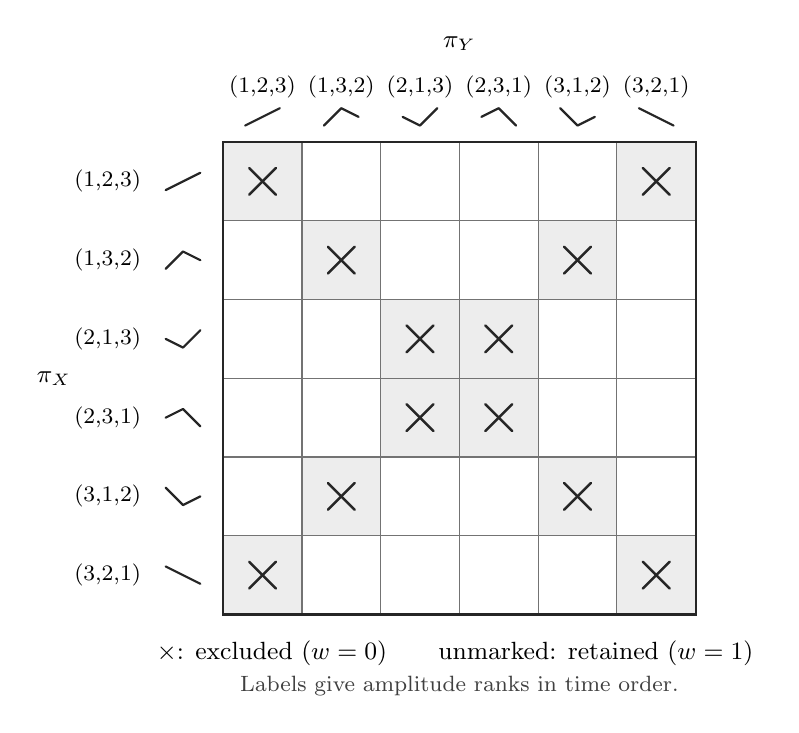
\begin{tikzpicture}[
    x=1cm, y=1cm,
    font=\small,
    pattern/.style={draw=black!85, line width=0.8pt, line cap=round,
                    line join=round},
    cross/.style={draw=black!85, line width=0.9pt, line cap=round}
]

% Shade excluded cells and draw the crosses.
\foreach \row in {1,...,6} {
    \foreach \col in {1,...,6} {
        \pgfmathtruncatemacro{\excluded}{
            (\row == \col) || (\row + \col == 7)
        }
        \ifnum\excluded=1\relax
            \fill[black!7] (\col-1,6-\row) rectangle (\col,7-\row);
            \draw[cross] (\col-0.67,6.33-\row)
                       -- (\col-0.33,6.67-\row);
            \draw[cross] (\col-0.67,6.67-\row)
                       -- (\col-0.33,6.33-\row);
        \fi
    }
}

% Six-by-six grid.
\draw[step=1, draw=black!55, line width=0.45pt] (0,0) grid (6,6);
\draw[draw=black!85, line width=0.8pt] (0,0) rectangle (6,6);

% Permutation labels and miniature ordinal patterns on both axes.
\foreach \i/\a/\b/\c in {
    1/1/2/3, 2/1/3/2, 3/2/1/3,
    4/2/3/1, 5/3/1/2, 6/3/2/1
} {
    % Column label and pattern: signal Y.
    \node[font=\footnotesize] at (\i-0.5,6.70) {$(\a,\!\b,\!\c)$};
    \draw[pattern] (\i-0.72,{6.10+0.11*\a})
                -- (\i-0.50,{6.10+0.11*\b})
                -- (\i-0.28,{6.10+0.11*\c});

    % Row label and pattern: signal X.
    \node[anchor=east, font=\footnotesize] at (-0.92,6.5-\i)
        {$(\a,\!\b,\!\c)$};
    \draw[pattern] (-0.73,{6.5-\i+0.11*(\a-2)})
                -- (-0.51,{6.5-\i+0.11*(\b-2)})
                -- (-0.29,{6.5-\i+0.11*(\c-2)});
}

\node at (3,7.25) {$\pi_Y$};
\node at (-2.15,3) {$\pi_X$};

% Optional legend: remove these nodes when supplying a separate caption.
\node[align=center] at (3,-0.49) {
    $\times$: excluded ($w=0$)\qquad unmarked: retained ($w=1$)
};
\node[font=\footnotesize, text=black!75] at (3,-0.91) {
    Labels give amplitude ranks in time order.
};
\end{tikzpicture}}
\caption{\removed{The outcomes available from wSMI. The crossed sections indicated are removed in the calculation in order to account for volume conduction.}\added{The six ordinal patterns for kernel length three, labelled by amplitude ranks in time order. Crosses identify identical and amplitude-reversed pairs excluded by both wSMI and wSD. The exclusion is intended to reduce common-source contributions.}}
\label{fig:mask}
\end{figure}


\section{Validation on sample data}
\added{\subsection{An exact negative-wSMI counterexample}
To show that negativity is a property of the population functional rather than only an estimation effect, modify the table in Eq.~\eqref{eq:zeroexample} to obtain $P=C/144$, where
\begin{equation}
C=\begin{pmatrix}
10&1&2&0&1&10\\
1&10&0&2&10&1\\
1&1&10&10&1&1\\
1&1&10&10&1&1\\
1&10&1&1&10&1\\
10&1&1&1&1&10
\end{pmatrix}.
\label{eq:counterexample}
\end{equation}
The four modified cells are all retained, and the modification preserves every row and column sum. Therefore $Q_{ij}=1/36$, $m=1/6$ and $z=2/3$ remain unchanged. Within $S$, two cells have count two, two have count zero and twenty have count one. Direct substitution gives
\begin{align}
W&=-\frac{11\log2}{36}\simeq-0.211795,\\
\operatorname{wSD}&=\frac{\log2}{36}\simeq0.019254.
\end{align}
The unweighted symbolic MI is approximately 0.551781 nats. All values are exact population quantities before decimal rounding. Dividing by $\log6$ gives the conventionally normalised measures and preserves the sign difference.

This distribution also has a finite time-series realisation. For each cell $(i,j)$, concatenate $C_{ij}$ paired blocks whose amplitudes equal the three ranks of symbols $i$ and $j$. With kernel three, delay one and stride three, the resulting 432-sample signals give exactly 144 paired symbols and reproduce $C$. Blocks are permuted together with a fixed random seed; no window crosses a block boundary. This construction establishes realisability for disjoint windows, and does not claim that an arbitrary ordinal table is attainable with overlapping windows in a stationary signal.

\subsection{Numerical checks and estimation bias}
We sampled 10,000 joint tables from a symmetric 36-cell Dirichlet distribution with concentration 0.4 per cell (seed 20261019). No table violated nonnegativity or the upper bound by unweighted symbolic MI, and 59 tables gave negative wSMI. The largest discrepancy in Eq.~\eqref{eq:correction} was $4.72\times10^{-16}$ nats. These checks test the implementation; the preceding proofs establish the distribution-wide results.

To examine the finite-sample null, we generated 200 independent pairs of independent standard Gaussian sequences at each of five lengths, with kernel three, delay one and overlapping windows. Population wSD is zero in this setting, but its mean plug-in estimate was 0.094992 nats for 100 samples and 0.000837 nats for 10,000 samples (Fig.~\ref{fig:synthetic}). Thus the proposed rescaling does not make the estimator unbiased. Overlapping windows are also not independent observations, so ordinary independent-cell uncertainty calculations should not be applied without justification.

\begin{figure*}[t]
\additioncolor
\centering
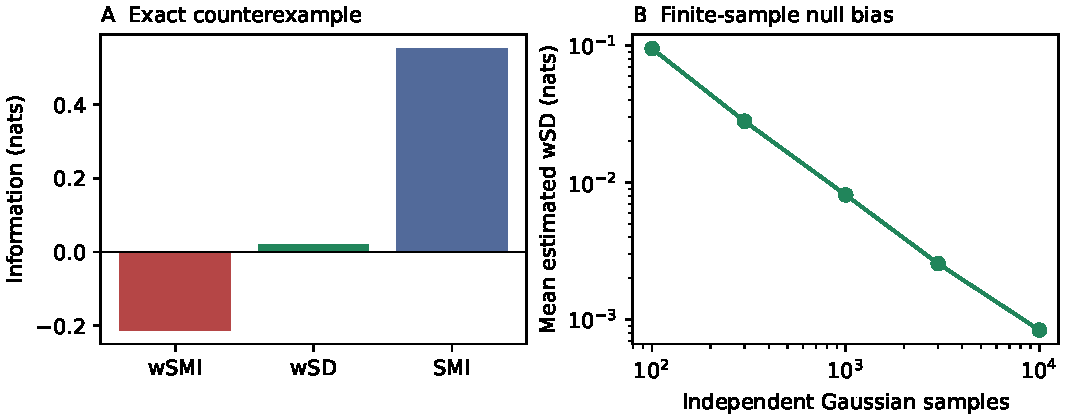
\includegraphics[width=.95\textwidth]{figures/synthetic_validation.pdf}
\caption{Exact and simulated validation. (A) The joint table in Eq.~\eqref{eq:counterexample} gives negative wSMI and positive wSD. (B) Mean estimated wSD for independent Gaussian sequences, using 200 replicates at each length. Its positive finite-sample bias decreases with sample length in this experiment.}
\label{fig:synthetic}
\end{figure*}

\subsection{Exploratory validation on public EEG}
We used the first five participants (S001--S005) and their two baseline recordings, eyes open (R01) and eyes closed (R02), from version 1.0.0 of the PhysioNet EEG Motor Movement/Imagery Dataset \cite{schalk2009dataset, schalk2004bci}. This fixed selection was made before inspecting the connectivity results. The recordings contain 64 EEG channels sampled at 160~Hz. Downloaded files were verified against the provider's SHA256 checksums; exact URLs and hashes are supplied with the analysis code.

Each recording was rereferenced to the common average and filtered continuously with a Butterworth bandpass designed using \texttt{scipy.signal.butter} with $N=4$ (an eighth-order bandpass), applied forward and backward using second-order sections. The lower cutoff was 0.5~Hz; the upper cutoff was $160/(3\tau)$~Hz. The primary delay was $\tau=4$ samples (25~ms; upper cutoff approximately 13.33~Hz); delays one and two were sensitivity analyses. The kernel was three throughout. The symbolic scale and lowpass convention follow the established wSMI methodology \cite{imperatori2019eeg}; this pilot does not reproduce a complete clinical wSMI preprocessing pipeline.

Five non-overlapping 10-second epochs began at 5, 15, 25, 35 and 45 seconds. Thus the first five seconds and all data from 55 seconds onward were excluded. Within each epoch, symbols were computed at every sample start, with no embedding across epoch boundaries. A pair was omitted if either ordinal window contained tied amplitudes; the joint table and both original marginals were computed from the same remaining pairs. There was no pseudocount or bias subtraction. All 2,016 distinct channel pairs were evaluated, giving 100,800 pair-epoch estimates for each delay. No channels or epochs were removed on the basis of connectivity values. There was no manual artifact rejection, ICA or source reconstruction, so artifacts and common-source effects remain possible explanations of individual estimates.

At the primary delay, wSMI was negative in 49,356 of 100,800 pair-epochs (48.96\%), whereas wSD ranged from 0.000813 to 0.621176 nats and never exceeded the corresponding unweighted symbolic MI. Each pair-epoch retained at least 1592 valid paired ordinal windows before the mask. Table~\ref{tab:negative} summarises the descriptive proportions by recording; Fig.~\ref{fig:eeg} shows all primary estimates. These pair-epochs share participants, electrodes and time, and must not be treated as 100,800 independent experimental units.

At delays one and two, respectively, 39.21\% and 49.23\% of pair-epochs gave negative wSMI; all wSD estimates again satisfied nonnegativity and the information bound. These proportions are descriptive and depend on the stated preprocessing and symbolic scale.

\begin{table}[t]
\additioncolor
\caption{Pair-epochs with negative wSMI at delay four. Each recording contributes 10,080 pair-epochs.}
\label{tab:negative}
\centering
\begin{tabular}{lrr}
\toprule
Participant & Eyes open (\%) & Eyes closed (\%)\\
\midrule
S001 & 57.3 & 53.5 \\
S002 & 57.1 & 42.1 \\
S003 & 65.5 & 57.2 \\
S004 & 53.7 & 26.3 \\
S005 & 40.0 & 37.0 \\
\bottomrule
\end{tabular}
\end{table}

For a reproducible illustration, the most negative primary wSMI occurred in S003R02, channels P5--PO7, in the epoch beginning at 15 seconds. Its wSMI was -0.154159 nats, while wSD was 0.063690 nats, with $m=0.166457$ and $z=0.616141$. The corresponding integer joint table is supplied as \texttt{eeg\_example\_counts.csv}. This example was selected after analysis to illustrate the sign contrast; it is not an independently selected hypothesis test.

As a descriptive null control, we circularly shifted one symbol sequence within each primary epoch for four prespecified homologous pairs (Fp1--Fp2, C3--C4, P3--P4 and O1--O2), using 99 shifts per pair-epoch, with seed 20261020. Shifts were sampled uniformly with replacement from integer offsets between 320 and $L-320$, where $L$ is the number of ordinal windows. This preserves each symbol sequence's cyclic structure while disrupting their original alignment. Across the 200 pair-epochs, the mean of the surrogate means was 0.018030 nats. The nonzero surrogate baseline reinforces the need for calibration; no significance or diagnostic claims are made. Circular shifts are an approximate control for dependent, potentially nonstationary data, not a guarantee of independence.

\begin{figure*}[t]
\additioncolor
\centering
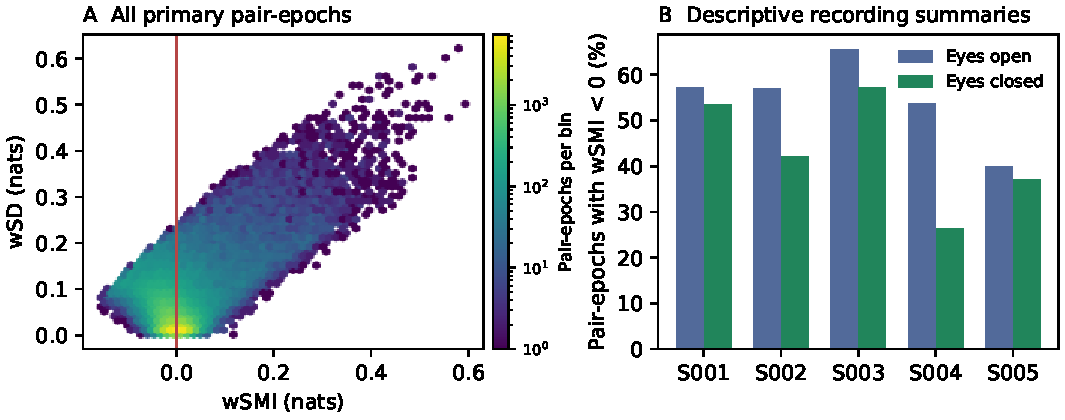
\includegraphics[width=.95\textwidth]{figures/eeg_validation.pdf}
\caption{Exploratory public-EEG results at kernel three and delay four. (A) All 100,800 pair-epoch estimates, with colour showing logarithmic bin counts and a vertical line at zero wSMI. (B) Descriptive percentages of negative wSMI within each recording. wSD remains nonnegative throughout; this numerical property is not evidence that all retained associations are physiological.}
\label{fig:eeg}
\end{figure*}
}
% Here's a toy system with negative wSMI.
% Wow in wSD it's positive how nice.
% Here's an experimental system with a problem.
% Here's how it looks now.

\added{\section{Implementation and limitations}
The accompanying Python package implements wSD, signed wSMI and ordinary symbolic MI from a joint count table, aligned ordinal symbols or two time series. It supports explicit logarithm bases and the conventional division by $\log(k!)$, and returns the retained joint and reference masses. Ordinal symbols use lexicographic amplitude ranks in time order. Ties can be rejected, omitted pairwise or resolved by temporal order; the default is rejection, so handling is never implicit. Nonfinite inputs are rejected. EEG filtering, rereferencing and artifact handling are external to the core estimator and are specified in the reproducible analysis script.

The computational core depends only on NumPy. Marginals are calculated before masking. Conditional KL is evaluated using a cancellation-resistant form, $\sum[r\log(r/s)-r+s]$, which equals KL for normalised probability vectors. A series expansion is used when $r$ is close to $s$. Signed wSMI is not clipped, and the implementation never manufactures nonnegativity by truncating its negative values. Tests cover the analytic example, its signal realisation, the partition identity, sparse and empty retained sets, units, ordinal coding, amplitude reversal, tied windows and invalid inputs.

The supplied replication materials include the fixed data-selection script, checksum manifest, analysis seeds, software versions, exact count tables, per-recording summaries and all pair-level empirical results. The package can be installed locally with \texttt{pip install .}; publication to a package index is a separate release step. The source repository is \url{https://github.com/KeenanDown/wSD}; the analysis and package described here are provided in the accompanying local revision.

The intended scope is selective dependence among retained interactions. A zero value when all deviations from independence lie in masked cells is therefore appropriate. Equation~\eqref{eq:zeros} also identifies the zero response when retained probabilities are a common multiple of the independence reference; whether that deviation is of interest depends on the application. Several empirical limitations remain. Nonnegativity is a property of the functional, not a finite-sample unbiasedness or significance guarantee. A nonnegative rescaling need not preserve rankings of connections, classification performance or resistance to source mixing. This five-participant EEG pilot supplies a real-data sign comparison, not an independent clinical validation. The sensitivity analyses change both the embedding delay and the associated filter cutoff, and therefore cannot isolate either effect. Future evaluation should compare estimators under matched preprocessing, calibrated surrogates, realistic common-source simulations and independent participant-level outcomes under prespecified hypotheses.
}

\section{Conclusion}

In this manuscript we introduced weighted symbolic divergence (wSD) as a potential successor to the weighted symbolic mutual information (wSMI). We demonstrated that where the wSMI is not always a positive quantity, \removed{wSD has the useful property that it is strictly positive for all possible distributions, while still accounting for the volume conduction effects that wSMI was designed to handle.}\added{wSD is nonnegative for every joint distribution. It is strictly positive precisely when retained mass is positive and the retained joint distribution is not proportional to the retained product of the original marginals. The measure preserves the exclusions used by wSMI, but a separate validation is needed to establish its sensitivity to genuine interactions and its resistance to volume conduction.}

Not only this, we saw that the wSD proposed has many natural and intuitive properties. It is bounded above by the raw mutual information between the two permutation variables, \removed{behaves locally like mutual information away from the weighted-out volume conduction nodes, and is intuitively familiar to the construction of mutual information as a KL-divergence.}\added{has a nonnegative quadratic expansion near independence, and follows the construction of mutual information as a KL divergence. Dependence confined to excluded cells is appropriately ignored by design. Its complete zero set also includes a uniform proportional change across retained cells, without a change in their relative distribution.}

\removed{In our analysis we also demonstrated that this new measure, wSD, is well behaved both on toy systems and experimental data: it is straightforward to calculate and exhibits behaviour familiar to wSMI while strengthening its mathematical foundations.}\added{Our analysis supplies an exact negative-wSMI/positive-wSD example, a signal-level realisation, a finite-sample null study, and an exploratory analysis of public EEG recordings. These results establish the proposed mathematical guarantees and demonstrate implementation on real data; they do not establish clinical usefulness, unbiased estimation, or superiority over wSMI. Appropriate surrogate calibration and independent evaluation remain necessary.}

We expect there may be other weighted information quantities which have similar symmetry-breaking behaviour beyond the wSMI. We believe that applying a similar rescaling procedure and using the KL-divergence will be a natural way to apply this method in many different domains.

\bibliographystyle{plain}
\bibliography{main.bib}

\end{document}
